\documentclass[10pt, margin=0.1in]{standalone}

\usepackage{braket}
\usepackage[compat=0.4]{yquant}
\useyquantlanguage{groups}
\usetikzlibrary{quotes, fit}

\begin{document}

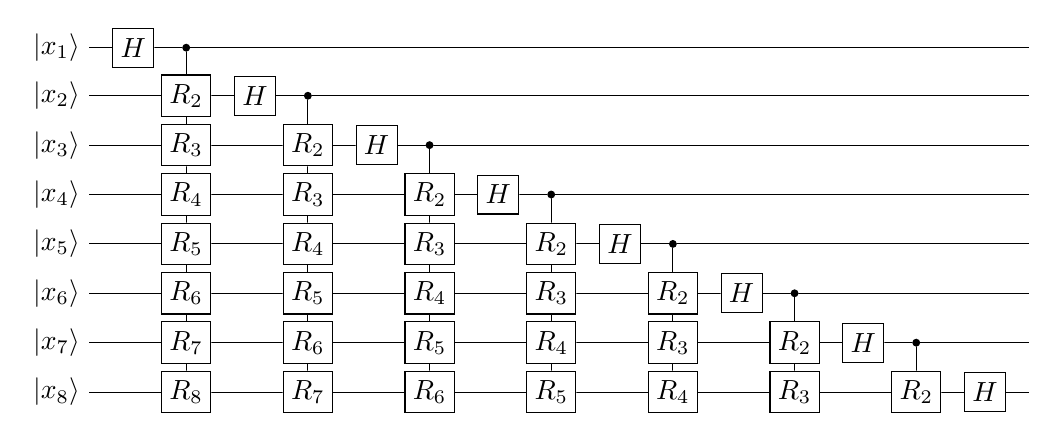
\begin{tikzpicture}
    \begin{yquant*}[loc/.style={style=blue, control style=blue}, nloc/.style={style=red, control style=red}]
    [drawing mode=quality]
    % registers
    qubit {$\ket{x_{\The\numexpr\idx+1}}$} q[8];
    
    hspace {2mm} -;
    h q[0];
    box {$R_{\The\numexpr\idx+2}$} q[1,2,3,4,5,6,7] | q[0];
    
    hspace {2mm} -;
    h q[1];
    box {$R_{\The\numexpr\idx+2}$} q[2,3,4,5,6,7] | q[1];

    hspace {2mm} -;
    h q[2];
    box {$R_{\The\numexpr\idx+2}$} q[3,4,5,6,7] | q[2];

    hspace {2mm} -;
    h q[3];
    box {$R_{\The\numexpr\idx+2}$} q[4,5,6,7] | q[3];

    hspace {2mm} -;
    h q[4];
    box {$R_{\The\numexpr\idx+2}$} q[5,6,7] | q[4];

    hspace {2mm} -;
    h q[5];
    box {$R_{\The\numexpr\idx+2}$} q[6,7] | q[5];

    hspace {2mm} -;
    h q[6];
    box {$R_{\The\numexpr\idx+2}$} q[7] | q[6];

    hspace {2mm} -;
    h q[7];
    hspace {2mm} -;

    \end{yquant*}
%     \node[fit=(left-0) (left-3) (right-0) (right-3),
% draw, inner sep=6pt, "reversed c-\textsc{not}"] {};
\end{tikzpicture}

\end{document}

